\documentclass[14pt, a4paper]{extarticle}
\usepackage[utf8x]{inputenc}
\usepackage[russian]{babel}
\usepackage{graphicx}
\usepackage{float}
\usepackage[outdir=./]{epstopdf}
\usepackage{booktabs}
\usepackage{tocvsec2}
\usepackage{amsfonts}
\usepackage{amsmath}
\usepackage[left=2cm,right=2cm,bottom=3cm,top=2cm]{geometry}

\graphicspath{ {./images/} }

\linespread{1.25}

\begin{document}

\thispagestyle{empty}

\begin{center}
\ \vspace{-4cm}

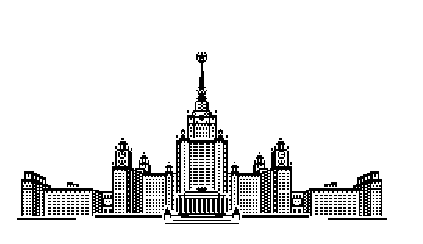
\includegraphics[width=0.5\textwidth]{msu}\\
{Московский государственный университет имени М.В. Ломоносова}\\
Факультет вычислительной математики и кибернетики\\
Кафедра автоматизации систем вычислительных комплексов

\vspace{5cm}

{\Large Долганов Станислав Викторович}

\vspace{1cm}

{\Large\bfseries
Метод поиска несоответствий границ объектов между результатом 2D-3D конвертации 
и используемыми картами глубины\\}

\vspace{1cm}

{\large ВЫПУСКНАЯ КВАЛИФИКАЦИОННАЯ  РАБОТА}
\end{center}

\vfill

\begin{flushright}
  \textbf{Научный руководитель:}\\
  к.ф-м.н.\\
  Д.С. Ватолин
\end{flushright}

\vfill

\begin{center}
Москва, 2016
\end{center}

\enlargethispage{4\baselineskip}

\newpage
% Аннотация (не более полстраницы) содержит формулировку задачи и основных результатов.

\textbf{Метод поиска несоответствий границ объектов между результатом 2D-3D конвертации 
и используемыми картами глубины}

\vspace{0.5cm}
Станислав Долганов
\vspace{0.5cm}

При создании полнометражных и любительских трехмерных фильмов с помощью 
конвертации отснятого в 2D материала достаточно часто возникают дефекты, 
связанные с качеством используемых карт глубины. Такого рода артифакты, 
даже если они находятся вне салиентных регионов,  могут заметно ухудшить 
восприятие смотрящего, и более того~---~вызвать головную боль. В дипломной
работе предлагается метод поиска объектов переднего плана, границы которых 
в стерео сцене не совпадают с действительностью, то есть объектов слитых 
с фоном. Предлагаемый метод извлекает информацию о движении в сцене и 
находит несоответствия конвертации между извлеченным движением и глубиной сцены.
Метод был применен на 39 полнометражных фильмах, что позволило найти 125 сцен с заметными несоответствиями границ объектов между картой движения и картой глубины, 
использованной при конвертации.

\vspace{2cm}

\textbf{Object boundaries inconsistencies detection method 
for 2D-3D (Two-Dimensional-Three-Dimensional)
conversion results and depth maps}

\vspace{0.5cm}
Stanislav Dolganov
\vspace{0.5cm}

The creation of S3D movies by converting 2D captured footage
often introduces depth-map inaccuracies. Such artifacts can
significantly degrade the viewing experience even if they occur
only in unsalient background objects.
In this paper we propose a method for detecting foreground
objects that are stuck to the background. Our method extracts
information about motion in the scene and detects conversionrelated
discrepancies between motion strength and depth. We
demonstrate the performance of the method by applying it
to 39 full-length converted 3D movies and by providing the
results of our analysis as well as examples of detected problem
shots.

\newpage
\addcontentsline{toc}{section}{Содержание}
\tableofcontents

\newpage
\section{Введение}
% Введение должно описывать предметную область, к которой относится задача, 
% решаемая в дипломной работе, содержать неформальное ее описание.

\subsection{Стереоскопическое видео и конвертация}

В наше время практически в каждом кинотеатре мира обязательно найдется сеанс в 3D. 
Такой интерес порождает повышенный спрос на стерео контент, однако развитие 
современных технологий производства 3D фильмов не способно в полной мере ему отвечать. 
Стандартный процесс создания контента происходит тремя возможными путями: 
\begin{itemize}
	\item съемка с помощью дорогостоящих стереоскопических систем камер,
	\item конвертация заранее отснятого двухмерного материала,
	\item использование компьютерной графики.
\end{itemize}
Последний подход относится к специфичной области мультипликационных фильмов, 
а также позволяет создавать различные спецэффекты на этапе постобработки. 
Съемка видео с помощью стерео камер требует постоянной каллибровки цветовых и 
геометрических парметров камер системы, что является не тривиальным процессом и 
потому зачастую приводит к некачественному контенту.  Учитывая последние разработки 
в области стерео конвертации~\cite{ndjiki2011depth,tolstaya2015depth}, которые 
заметно улучшили визуальное качество результата, а также сравнительно меньшие 
затраты на производство, легко заметить, что многие киностудии предпочитают 
конвертацию остальным подходам. В данном факте можно убедиться, если посмотреть 
на ежегодные соотношения конвертированных и отснятых фильмов за последние 60 лет~\cite{realorfake}.

\subsection{Проблемы конвертации} 

Хотя существующие программные инструменты на порядок облегчают различные 
этапы конвертации видео, сам процесс остается достаточно трудоемким и 
далеким от автоматизации. Майк Сеймор в своем обзоре~\cite{seymour2012art} 
описывает основные проблемы генерации стереовидео по исходному 2D материалу:
\begin{itemize}
	\item Эффект параллакса --- означает, что для генерации второго ракурса 
	необходимо заполнять области сцены, которые не видны на исходном ракурсе. 
	Основная проблема заключается в выборе материала для заполнения открывающихся 
	областей, который не вызывал бы дискомфорта при просмотре и был бы стабильным во времени.
	\item Эффект кулисности --- означает, что для объектов переднего плана необходимо 
	сгенерировать различную глубину для различных частей объекта, что позволит сделать 
	объект рельефным, иначе при просмотре сцены объект будет казаться плоским, 
	что противоречит реальной жизни.
	\item Эффект отжимающего действия рамки --- возникает, когда объекты с отрицательным 
	параллаксом, то есть такие объекты, которые при просмотре кажутся ближе к зрителю, 
	чем плоскость экрана, пересекают рамку экрана. Появлятся невозможная в реальной 
	жизни ситуация, когда часть объекта находится перед нами, а оставшаяся часть скрыта 
	более удаленной рамкой. Наиболее точно такую ситуацию можно объяснить следующим 
	образом --- представить, что объект находится перед окном и начинает двигаться 
	от центра окна к его краю, затем часть объект пересекающая границу окна пропадает.
	\item Агрессивная величина параллакса --- может проявляться различными путями. 
	Первый возможный вариант---это большие значения как положительного, так и 
	отрицательного параллакса в сцене, что влечет за собой большой разброс объектов 
	в сцене, тяжело переносится зрителем и может стать причиной головной боли. 
	Второй вариант заключается в значительном изменении отрицательного и положительного 
	параллаксов между двумя соседними сцены. Такая ситуация требует от зрителя 
	адаптироваться к каждой сцене, что также может сильно утомлять.
	\item Некачественная карта глубины. Общее качество карты глубины, которая является 
	необходимой частью процесса конвертации, прямым образом влияет на результат, 
	поэтому очень важно контролировать соответствие карты действительности, 
	что касается как верного выбора расположения объектов по глубине в сцене, 
	так и точных границ объектов.
\end{itemize}

Эффект кулисности и остальные дефекты карт глубины, которые возникают в процессе 
конвертации из 2D в 3D часто ухудшают общее восприятие зрителя от просмотра фильма. 
Наиболее значимые проблемы создают объекты, находящиеся в салиентных областях 
сцены, границы по движению которых не совпадают с границами по глубине, то есть 
таких объектов, которые движутся про пространству сцены не равномерно или деформируются, 
что не возможно в реальной жизни. Исследования в этой области~\cite{jung2012visual,li2014visual} подтверждают ухудшение состояния группы людей, которые смотрят такого рода стереовидео.

\subsection{Полуавтоматический контроль качества конвертации}

\begin{figure}[!h]
	\begin{minipage}[b]{1.0\linewidth}
		\centering
		\centerline{ 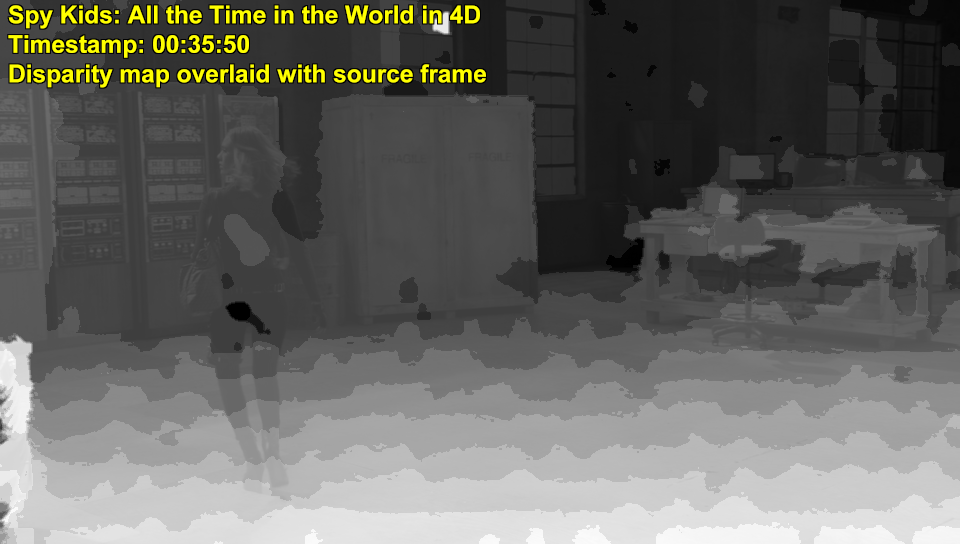
\includegraphics[width=0.7\textwidth]{example_depth} }
	\end{minipage}
	\begin{minipage}[b]{1.0\linewidth}
		\centering
		\centerline{ 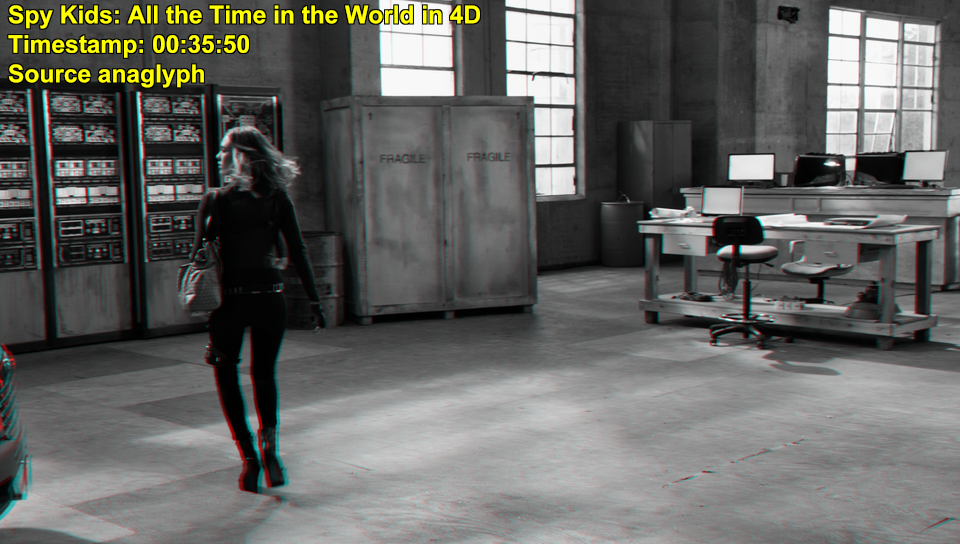
\includegraphics[width=0.7\textwidth]{example_anaglyph} }
	\end{minipage}
    \caption{Пример найденной с помощью предлагаемого метода сцены, содержащей дефект: объект переднего плана оказался слитым с фоном. Создатели фильма забыли нарисовать тело актрисы на карте глубины, поэтому сцена демонстрирует невозможную ситуацию и может вызвать визуальный дискомфорт. На верхнем изображении показана карта диспаратности поверх исходного ракурса, на нижнем --- исходная сцена в анаглифе. }
	\label{fig:example}
\end{figure}


Основной целью данной дипломной работы является создание программного инструмента, 
который позволит автоматически оценить качество используемых карт глубины,
что в свою очередь позволит киностудиям создавать более качественный контент. 
Частой практикой киностудии является разделение фильма на крупные части, которые 
затем отправляются на конвертацию в специализированные компании. Такой подход 
ухудшает качество, так как компании не знают о результатах работы друг друга. 
Основной выигрыш для киностудии---это уменьшение времени, которое понадобиться 
для конвертации, однако из-за сжатых сроков, а так же ручного тестирования 
качества результата, часто возникают такие сцены как на Рис.~\ref{fig:example}. 
Предлагаемый программный инструмент позволит проводить проверку в полуавтоматическом 
режиме, что несомненно повысит как качество, так и время производства.
В качестве входных данных предлагаемому алгоритму требуются стерео видеопоследовательность 
и опционально карты глубины, используемые во время конвертации в 3D формат данной видеопоследовательности. В случаях, когда информация об используемых картах 
глубины недоступна, метод оценивает карту диспаратности с помощью~\cite{simonyan2008fast,zhang2014100+}. Он находит дефекты сравнивая 
для каждого отдельного кадра границы карты глубины/диспаратности с границами карты 
амплитуды движения. Такой подход позволяет находить движущиеся объекты, которые 
частично или полностью отсутствуют на оцениваемой карте глубины. Так как не существует 
общепринятого быстрого и качественного алгоритма оценки векторов движения, было принято 
решение использовать в качестве такого алгоритма~\cite{simonyan2008fast}, который 
применяется к последовательности левых ракурсов. Затем полученная последовательность 
оценненых карт амплитуды движения итеративно улучшается с помощью временных и 
пространнственных фильтраций~\cite{fecker2007time,matyunin2011temporal,he2013guided}. 
Результирующая оценка для каждого кадра высчитывается, как величина несоответствия 
глубины и движения. Оценка для сцены высчитывается, как средневзвешенная оценка 
соответствующих кадров, где веса высчитываются на основании доверия 
к оцененными векторам движения.

\newpage
\section{Постановка задачи}
% Постановка задачи должна содержать формулировку задачи в рамках определенной модели 
% предметной области, к которой относится решаемая задача, требования к искомому решению 
% в терминах используемой модели предметной области.

\subsection{Неформальная постановка задачи}

Пусть имеются две видеопоследовательности, одна из которых снята на камеру, а вторая получена с помощью конвертации, таким образом, что видеопоследовательности вместе являтся ракурсами стереоскопического видео. Также опционально может иметься видеопоследовательность, состоящая из карт глубины, использованных для конвертации. Требуется определить наличие объектов слитых с фоном, то есть объектов, границы которых по глубине не совпадают с действительностью.

\subsection{Формальная постановка задачи}

Обозначения:

\textit{Пиксель} $p$ --- тройка $<p_r,p_g,p_b>$ целых чисел от 0 до 255, определяющих цветовые компоненты в пространстве RGB.

\textit{Изображение} $I$ --- матрица размера $h \times w$ из пикселей.

\textit{Видеопоследовательность} $\{I_t\}_{t=0}^N$ --- конечный упорядоченный набор изображений (кадров) одинаковых размеров.

\begin{figure}[!h]
	\begin{minipage}[b]{1.0\linewidth}
		\centering
		\centerline{ 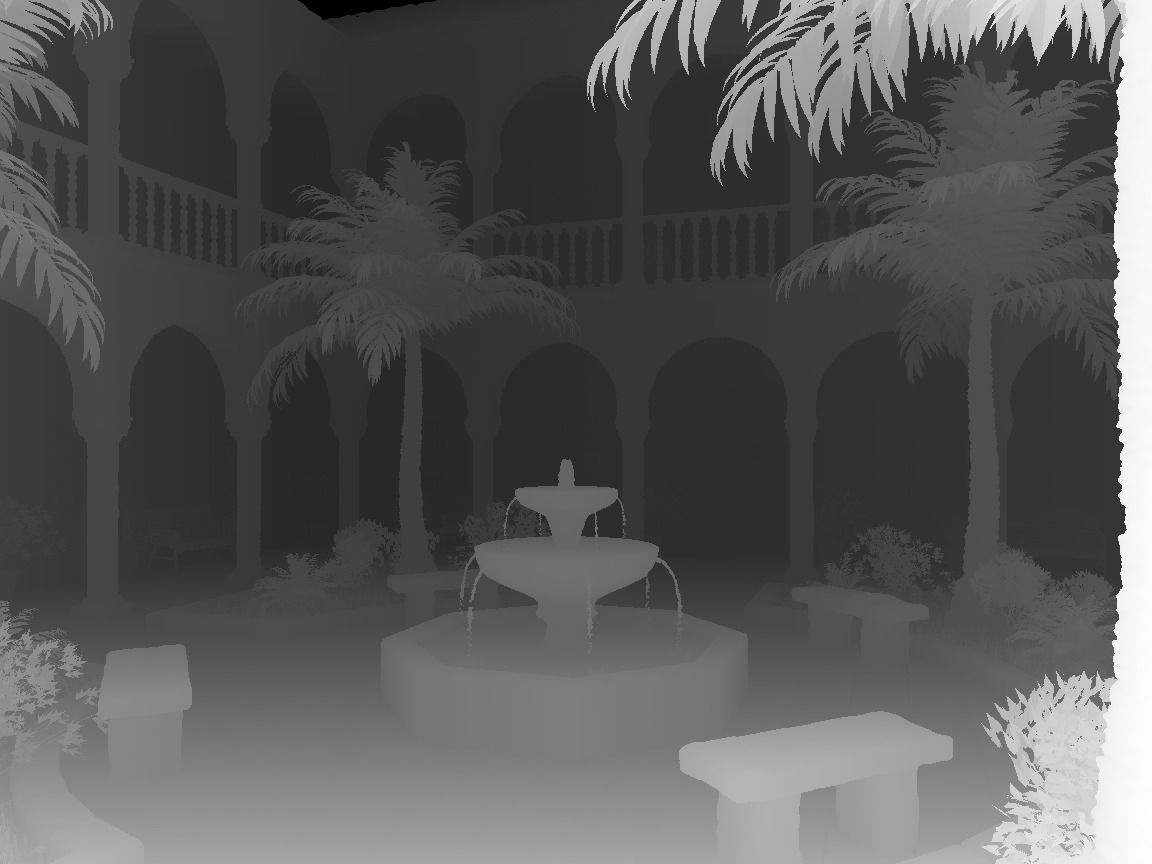
\includegraphics[width=0.7\textwidth]{depth_map_example} }
	\end{minipage}
    \caption{Пример карты глубины.}
	\label{fig:depth_map_example}
\end{figure}


\textit{Карта глубины} $D$ --- матрица размера $h \times w$, состоящая из чисел от 0 до 255,
определяющая расстояние от позиции смотрящего до всех объектов в сцене, 
где значение 255 соответствует положению смотрящего, 128 плоскости экрана, 
а 0 --- <<бесконечности>>. Пример Рис.~\ref{fig:depth_map_example}.

\textit{Последовательность карт глубины} $\{D_t\}_{t=0}^N$ --- конечный упорядоченный 
набор карт глубины одинаковых размеров, которые используются алгоритмом конвертации 
для извлечения информации о расположении объектов в сцене.

\textit{Конвертированное стереовидео} $𝑆$ --- упорядоченная пара видеопоследовательностей 
($\{L_t\}_{t=0}^N$,$\{R_t\}_{t=0}^N$), совпадающих по количеству кадров и размеру кадров, 
где $\{L_t\}_{t=0}^N$ --- это снятая видеопоследовательность, а $\{R_t\}_{t=0}^N$ --- 
полученная на основании $\{L_t\}_{t=0}^N$ и $\{D_t\}_{t=0}^N$, сконвертированная последовательность. 
Видеопоследовательности называются левым и правым ракурсом соответственно.

\textit{Оценка} $q$ --- действительное неотрицательное число $q \in \mathbb{R}^{+} \cup \{0\}$, 
пропорциональное величине заметности артифакта в стереопаре.

Постановка задачи:

\begin{enumerate}
	\item На вход алгоритму, реализующему разрабатываемый метод, подаётся конвертированное стереовидео $𝑆$, а также дополнительно может быть передана последовательность карт глубины $\{D_t\}_{t=0}^N$.
	\item Выходом алгоритма является набор оценок $\{q_t\}_{t=0}^N$, соответствующих кадрам входящей стерео видеопоследовательности.
\end{enumerate}

\subsection{Требования к методу}

Разрабатываемый метод должен быть применим для анализа полнометражных стереоскопических фильмов. Соответственно, он должен удовлетворять следующим требованиям:

\begin{itemize}
	\item Способность находить сцены с заметными артифактами, 
	находящимися в областях салиентного движения.
	\item Низкая доля ошибок первого рода (пропуск сцены) при приемлемой доле 
	ошибок второго рода (ложное срабатывание). Ошибки второго рода менее существенны, 
	так как, если ложных срабатываний не очень много, их можно исключить 
	при ручном просмотре обнаруженных сцен.
	\item Высокая скорость работы на видеопоследовательностях высокого разрешения 
	вплоть до $1920 \times 1080$. Требуется для того, чтобы анализ 
	полнометражного стереоскопического фильма занимал приемлемое время.
	\item Устойчивость к другим типам артифактов, главным из которых является отсутствие глубины в сцене (сцена выглядит плоской, либо присутствует только некоторый градиент по глубине).
\end{itemize}

\subsection{Цели дипломной работы}

Целью дипломной работы является разработка метода, решающего поставленную задачу 
с минимальной долей ошибок первого рода (артифакт не обнаружен) и 
с приемлемой долей ошибок второго рода (ложное срабатывание).

В рамках дипломной работы предполагается решить следующие задачи:

\begin{enumerate}
	\item Провести обзор предметной области алгоритмов оценки качества конвертированного стереовидео.
	\item Разработать метод поиска несоответствий границ объектов между результатом 2D-3D конвертации 
	и используемыми картами глубины, учитывая требования данной задачи.
	\item Разработать алгоритм, реализующий метод, и провести его экспериментальную оценку на соответствие требованиям решаемой задачи.
	\item Произвести массовый анализ реальных стереоскопических фильмов на предмет наличия движущихся объектов, слитых с фоном.
\end{enumerate}


\newpage
\section{Обзор предметной области}
% Обзор должен содержать явно сформулированные цели и критерии сравнения, которые 
% должны коррелировать с требованиями к искомому решению исходной задачи. 
% В конце обзора должны быть сформулированы выводы.

\subsection{Методы оценки качества 2D видеопоследовательностей}

Многие годы ислледователи изучали качество 2D видеопоследовательностей. 
Wang~\cite{wang2006survey} предложил исчерпывающий обзор основных подходов в данной области.
Самым популярным методом является \textbf{Peak-Signal-to-Noise-Ratio (PSNR)}:
\begin{equation*}
	MSE = \frac{\sum_{i=0}^{h}\sum_{j=0}^{w}[I(i, j) - I'(i, j)]^2}{h \cdot w},
\end{equation*}
\begin{equation}
	PSNR = 20 \cdot \log_{10}(\frac{255}{MSE}),
\end{equation}
где $I$, $I'$ два изображения, которые сравниваются. Чем выше значение $PSNR$, 
тем больше похожи изображения, $PSNR \equiv +\infty$ соответствует одинаковым изображениям. 
Метод \textbf{Structural Similarity Index (SSIM)} многими ислледователями был принят, 
как основной метод оценки качества приближающий субъективную оценку. Данный метод встречается
практически в каждой статье и описывается следующим уравнением:
\begin{equation}
	SSIM = \frac{(2\bar{x}\bar{y} + C_1)(2\sigma_{xy} + C_	2)}{[\bar{x}^2 + \bar{y}^2 + C_1](\sigma_x^2 + \sigma_y^2 + C_2)},
\end{equation} 
где $\bar{x}$, $\bar{y}$, $\sigma_x$, $\sigma_y$, $\sigma_{xy}$ --- средние значение 
для первого изображения, средние значение для второго изображения, дисперсия для $x$, 
дисперсия для $y$, ковариация $x$ и $y$; $C_1$, $C_2$ --- константы. Значение $SSIM$ 
высчитывается с помощью скользящего окна размером $11 \times 11$ с весами Гауссового ядра, 
а итоговое значение для двух изображений --- это среднее по всем высчитанным окнам.

\subsection{Методы оценки качества стереоскопического видео}

Основными направлениями исследований в области оценки качества стереоскопического видео 
являются множественные несоответствия между ракурсами и временная стабильность 
динамического диапазона глубины. Voronov в соавторстве~\cite{voronov2012towards} предложил
способ нахождения разницы между ракурсами по цвету, резкости, 
а также различных геометрических искажений. В статье~\cite{akimov2012automatic} авторами 
был предложен метод нахождения перепутанных ракурсов в стереовидео. 

Артифакты, влияющие на качество конвертированного стереоскопического видео, более 
разнообразны и менее изучены в научных кругах. Bokov в соавторстве~\cite{bokov2014automatic} 
предложил алгоритм поиска трех основных проблем, возникающих при конвертации:
\begin{itemize}
	\item Резкость границ объектов,
	\item Эффект кулисности,
	\item Плоские сцены.
\end{itemize}
Ожидаемо, данный алгоритм подходит для обнаружения проблем только для тех объектов, 
которые присутствуют на карте глубины. В данной дипломной работе предлагается 
дополнительный метод, расширяющий возможности оценки качество конвертированного стереовидео,
позволяющий находить объекты переднего планы частично или полностью отсутствующие
на используемых картах глубины.

\subsection{Обзор базовых алгоритмов}

Предлагаемый метод является композицией двух крупных областей исследований: извлечение структуры 
сцены на основании информации о движении, а также алгоритмов сопоставления краев и контуров 
между двумя картами границ. Обе области достаточно хорошо изучены.

Многие методы извлечения структуры сцены из движения предполагают минимизацию функции энергии
с членом, отвечающим амплитуде движения, извлеченной из сцены. Яркий 
представитель~\cite{zhang2009consistent} дополнительно учитывает ограничение, 
обеспечивающее временную стабильность, а также уточняют положение объектов с помощью ротации 
в пространстве плоскостей, соответствующих цветовым сегментам кадра, в сторону уменьшения энергии.
Такой подход позволяет извлекать карты глубины высокого качества, обладающих временной стабильностью.
Однако временная сложность алгоритма не подходит для решения прикладных задач, в частности 
для анализа полнометражного стереоскопического фильма. Недавно предложенный 

A recently proposed edge-aware filter~\cite{he2013guided} allows us to employ a less sophisticated approach: we obtain a rough motion-strength map through a block-based motion-estimation algorithm~\cite{simonyan2008fast} and then enhance the result using edge-aware convolution.
To address the contour-matching problem, several very precise methods of closed-contour matching have recently appeared. For instance, Xu et al.~\cite{xu20092d} proposed a method based on contour-flexibility descriptors. Extension to open contours is possible but requires extraction of problem edges using a watershed transform. This transform leads to significant growth in second-order errors, however. Felzenszwalb et al.~\cite{felzenszwalb2007hierarchical} proposed a competing approach that uses a hierarchical shape tree. Unfortunately, this method is not extensible to discontinuous contours, which are critical to our case because motion extraction is imperfect and the resulting motion-edge maps contain numerous discontinuities. Thus, we employ a less precise but more robust approach to input-contour-map inaccuracies that is similar to a distance transform~\cite{borgefors1986distance}.

\newpage
\section{Предложенный метод}

%\begin{figure}[!h]
	\begin{minipage}[b]{0.49\linewidth}
		\centering
		\centerline{ 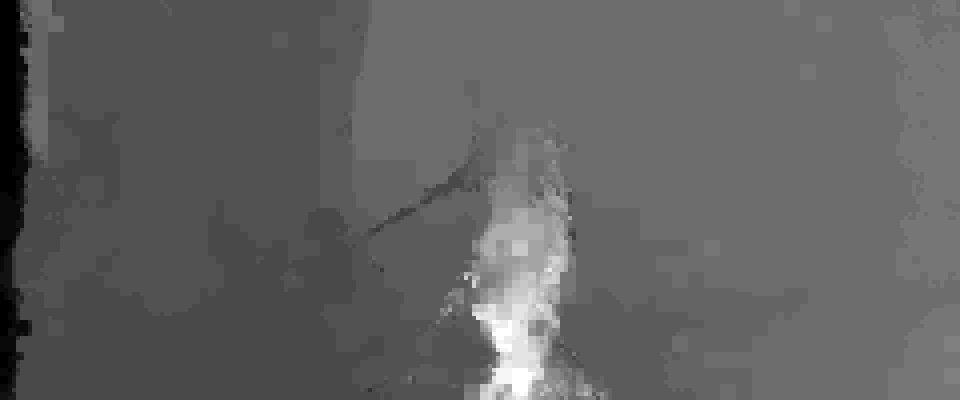
\includegraphics[width=\linewidth]{motionx} }
		\centerline{\scriptsize{(a) Horizontal-motion strength map}}\medskip
	\end{minipage}%
	\hfill
	\begin{minipage}[b]{0.49\linewidth}
		\centering
		\centerline{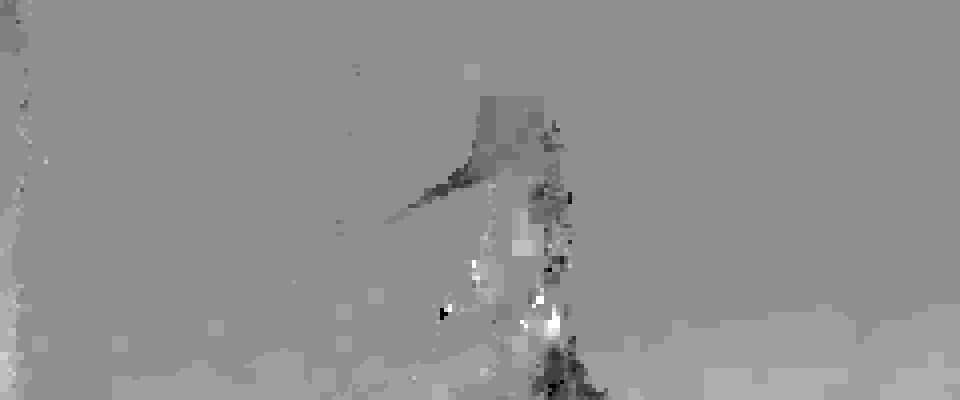
\includegraphics[width=\linewidth]{motiony} }
		\centerline{\scriptsize{(b) Vertical-motion strength map}}\medskip
	\end{minipage}
	\begin{minipage}[b]{0.49\linewidth}
		\centering
		\centerline{ 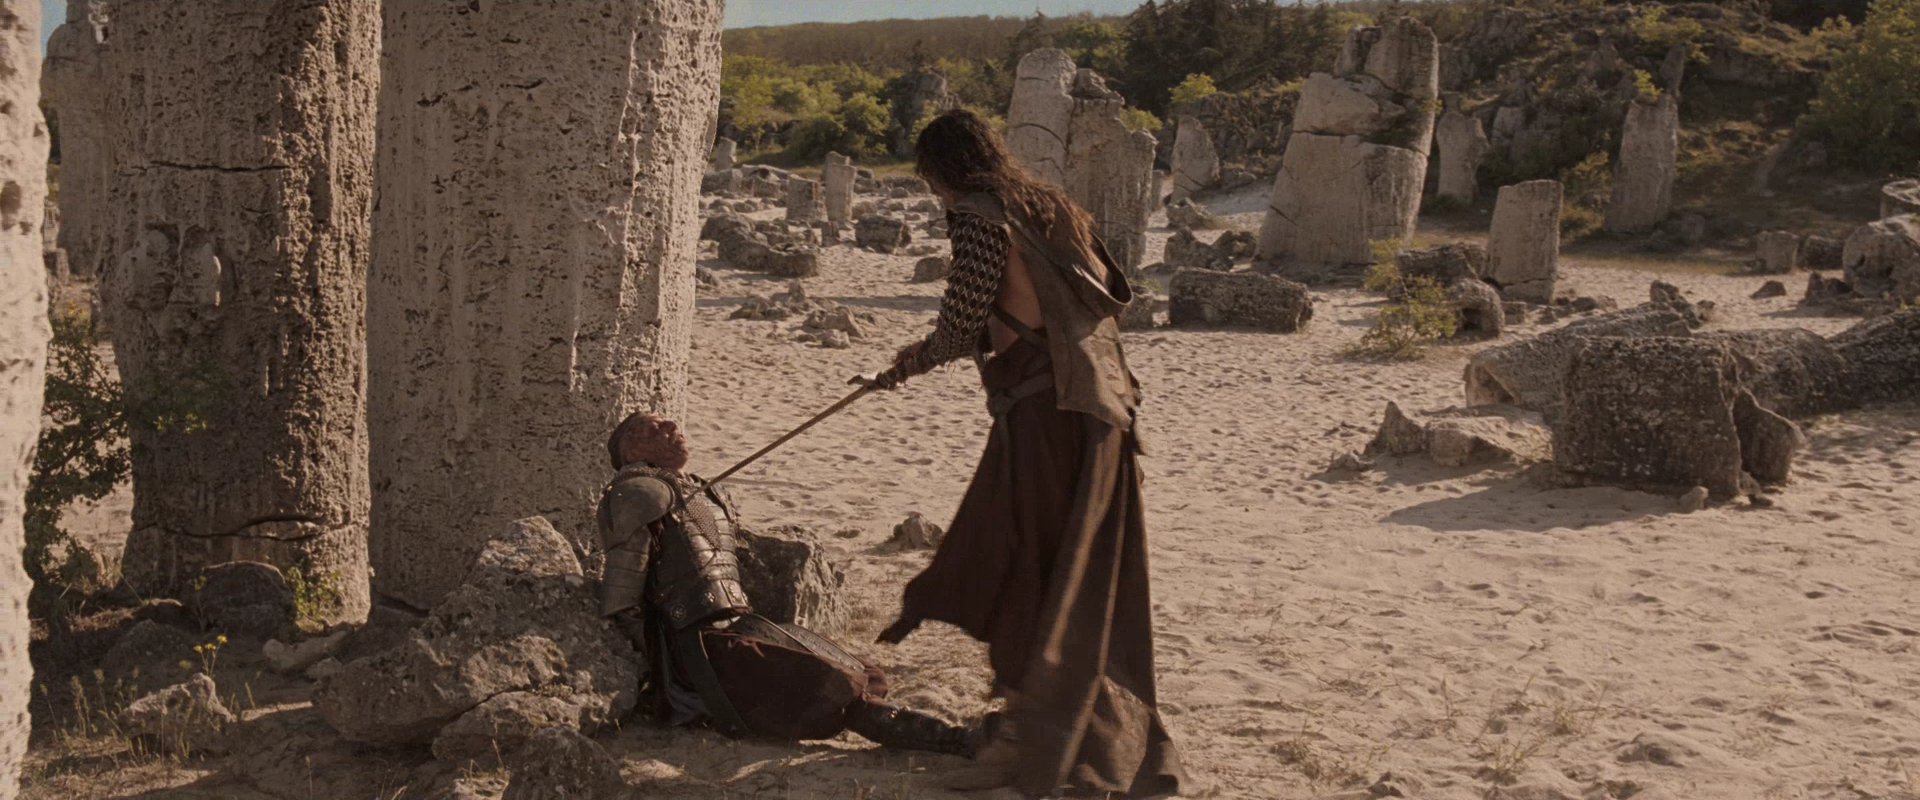
\includegraphics[width=\linewidth]{src} }
		\centerline{\scriptsize{(c) Source left view}}\medskip
	\end{minipage}%
	\hfill
	\begin{minipage}[b]{0.49\linewidth}
		\centering
		\centerline{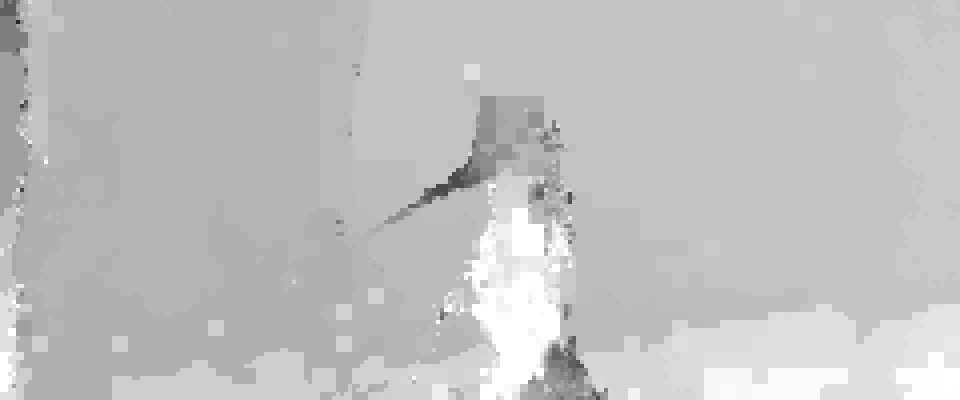
\includegraphics[width=\linewidth]{merged} }
		\centerline{\scriptsize{(d) Overall motion-strength map}}\medskip
	\end{minipage}
	\begin{minipage}[b]{\linewidth}
	\caption{Example maps of horizontal~(a) and vertical~(b) motion extracted
        using a block-based motion-estimation algorithm~\cite{simonyan2008fast} for the source frame~(c).
        The results  are combined into an overall motion-strength map~(d).}
    \label{fig:merged}
    \end{minipage}
\end{figure}



\newpage
\section{Экспериментальная оценка}

\newpage
\section{Программная реализация}

\newpage
\section{Заключение}

\subsection{Результаты работы}

\subsection{Направления для дальнейшего исследования}

\subsection{Публикации и гранты}

По теме данной работы были сделаны следующие публикации:

\begin{itemize}
	\item Dolganov S. et al. Detection of stuck-to-background objects in converted S3D movies // 3D Imaging (IC3D), 2015 International Conference on. – IEEE, 2015. – С. 1-6.
	\item Долганов С. В. <<Метод поиска несоответствий границ объектов между результатом 2D-3D конвертации и используемыми картами глубины>> // XXIII Международная конференция студентов, аспирантов и молодых ученых <<Ломоносов-2016>>, стр. 11-13.
\end{itemize}

Также работа была частично поддержана грантом РФФИ № 15-01-08632-а.

\newpage
\section{Приложения}

\newpage
%\section*{Список литературы}
\addcontentsline{toc}{section}{Список литературы}
\bibliographystyle{gost2008}
\bibliography{dipbib}

\end{document} 